\documentclass{standalone}
\usepackage[utf8]{inputenc}
\usepackage[T1]{fontenc}
\usepackage{ngerman}
\usepackage{xcolor}
\usepackage{fixltx2e}
\usepackage{tikz}
\usepackage{titlesec}
\usepackage{booktabs}

\usetikzlibrary{shapes,positioning,arrows,backgrounds,calc,fit}
%\usetikzlibrary{shapes.geometric,backgrounds,positioning-plus,node-families,calc}
%\usetikzlibrary{shapes.geometric,backgrounds,calc}

% http://www.texample.net/tikz/examples/flowchart/

\definecolor{fhgg}{RGB}{23,156,125} % green
\definecolor{fhgo}{RGB}{235,106,10} % orange
\definecolor{fhgdb}{RGB}{0,110,146} % dark blue
\definecolor{fhglb}{RGB}{37,186,226} % light blue
\definecolor{fhgy}{RGB}{177,200,0} % yellow green

\newcommand{\cfile}{fhglb!20!white}
\newcommand{\csel}{fhgo!20!white}
\newcommand{\cbuf}{fhgg!20!white}
\newcommand{\calg}{fhgy!20!white}

\tikzset{
	every node/.style = { align = center, draw },
	io/.style = { signal, signal to=south, signal pointer angle=150, fill=\cfile, minimum width=20mm },
	alg/.style = { rectangle, minimum width=15mm, minimum height=6mm, fill=\calg },
	clr/.style = { draw=none },
	head/.style = { clr, font=\large },
	buf/.style = { cylinder, shape aspect=.5, fill=\cbuf },
	op/.style = { circle, fill=\calg },
 	cfg/.style = { buf, font=\scriptsize },
	dsc/.style = { clr, font=\scriptsize, align=left, anchor=west },
	blk/.style = { inner sep=3mm, color=fhgdb, append after command={
		\pgfextra{\let\TikZlastnode\tikzlastnode}
		node [draw=none,anchor=north west,text=fhgdb] (blk-\TikZlastnode) at (\TikZlastnode.north west) {#1}
	}},
}



\tikzset{
	sel/.style = { diamond, font=\small, shape aspect=4, fill=\csel, append after command={
		\pgfextra{\let\TikZlastnode\tikzlastnode}
		node [draw=none,anchor=north east,outer sep=-0.5mm] at (\TikZlastnode.south west) {\tiny NONE}
		node [draw=none,anchor=north west,outer sep=-0.5mm] at (\TikZlastnode.south east) {\tiny MEL}
  }}
}

\begin{document}
\pagestyle{empty}
\thispagestyle{empty}
\sffamily

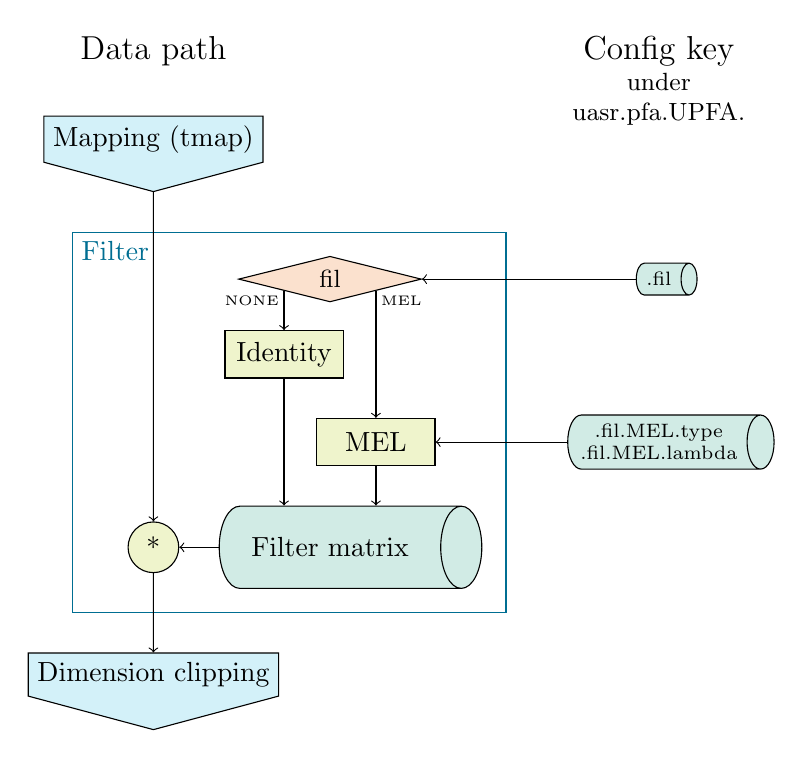
\begin{tikzpicture}[node distance=5mm]
\node (sel)   [sel]   {fil};

\node (none)  [alg,below=of sel.south west] {Identity};
\node (mel)   [alg,below=of sel.south east|-none.south] {MEL};
\draw[->] (sel.south west) -- (none);
\draw[->] (sel.south east) -- (mel);

\node (mat)   [buf,below=of sel|-mel.south,inner sep=4mm] {Filter matrix};
\draw[->] (none) -- (none|-mat.north);
\draw[->] (mel)  -- (mel|-mat.north);

\node (mul)   [op,left=of mat]    {*};
\draw[->] (mat)  -- (mul);

\coordinate (fill) at ($(mul.west)-(4mm,0)$);
\node (fil)  [blk=Filter,fit=(sel)(mel)(mat)(mul)(fill)] {};

\node (in)    [io,above=of mul|-fil.north]   {Mapping (tmap)};
\node (out)   [io,below=of mul|-fil.south]   {Dimension clipping};
\draw[->] (in)   -- (mul);
\draw[->] (mul)  -- (out);

\node (phead) [head,above=of in] {Data path};
\node (chead) [head,right=of fil.east|-phead.north,anchor=north west] {Config key \\ \small \begin{tabular}{c}under \\ uasr.pfa.UPFA.\end{tabular}};
%\node (dhead) [head,right=of chead.north east,anchor=north west] {Description};
%\coordinate (chead) at ($(trf.east)+(15mm,0)$);

\draw[<-] (sel)  -- (chead|-sel)  node[cfg]{.fil};
\draw[<-] (mel)  -- (chead|-mel)  node[cfg]{.fil.MEL.type \\ .fil.MEL.lambda};

\end{tikzpicture}

\end{document}
